\documentclass[9pt]{article}
\usepackage{amsmath,amsfonts,amssymb,times}
\usepackage{graphicx,color,tikz,pgfplots}
\usepackage[paperwidth=7.6cm,paperheight=5.3cm,lmargin=0in,rmargin=0in,tmargin=4pt,bmargin=0.in]{geometry}
\usepackage{bm}
\usetikzlibrary{arrows,shadings,shapes.arrows,decorations.pathreplacing,calc}
\usepgfplotslibrary{fillbetween}


\pagestyle{empty}
\pgfplotsset{compat=newest}
\definecolor{applered}{RGB}{255,8,0}
\definecolor{azure}{RGB}{0,127,255}
\definecolor{violet}{RGB}{159,0,255}

\pgfdeclareverticalshading{rainbow}{100bp}
{color(0bp)=(applered); color(25bp)=(red); color(40bp)=(yellow);
  color(47bp)=(green); color(51bp)=(cyan); color(60bp)=(blue);
  color(65bp)=(violet); color(100bp)=(violet)} 
                          
\newlength{\h}
\newlength{\rad}
\setlength{\h}{2.5cm}
\setlength{\rad}{1.5pt}

\begin{document}
\centering
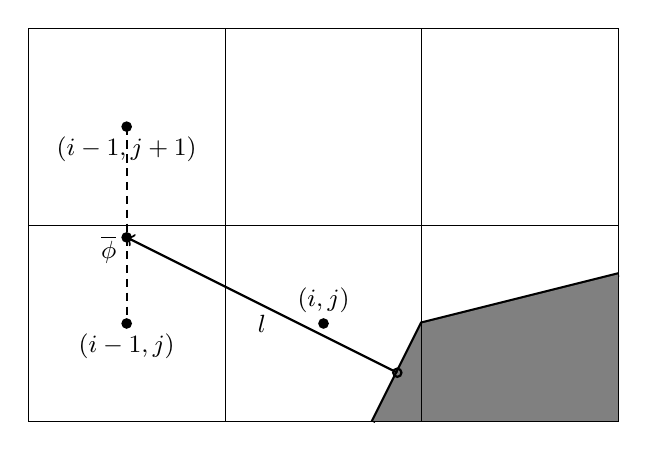
\begin{tikzpicture}[
    gridstyle/.style={thin,black},
    nodeCenterStyle/.style={thick,black,fill},
    nodeFaceStyle/.style={thick,black},
    VoFStyle/.style={font=\small,anchor = north west},
    surfaceStyle/.style={ultra thick,black},
    volumeStyle/.style={thick,densely dashed,black},
    surfaceFill/.style={},
    braceStyle/.style={thick,decorate,decoration={brace,amplitude=4pt,raise=2pt}},
    alphaStyle/.style={font=\small,anchor=east,xshift=-4pt},
    hTopStyle/.style={font=\small,anchor=east,yshift=4pt},
    hLeftStyle/.style={font=\small,anchor=east,xshift=-4pt},
    betaStyle/.style={font=\small,anchor=west,xshift=4pt},
    EBStyle/.style={font=\small,anchor=south,yshift=4pt},
    kappaStyle/.style={font=\small,anchor=center},
    normalStyle/.style={font=\small,->,thick,black},
    gradientStyle/.style={font=\small,->,thick,black},
    surfaceCharge/.style={font=\small,yshift=2pt},
    phiStyle/.style={font=\small,anchor=south},
  ]

  %EB
  \path[name path=baseline] (1.5\h,\h) -- (3\h,\h);
  \draw[surfaceStyle,name path=surface] (1.75\h,\h) -- (2\h,1.5\h) -- (3\h,1.75\h);
  \tikzfillbetween[of=surface and baseline,on layer=,every segment/.style={surfaceFill}] {black!50!white};

  %% Grids and nodes
  \draw[step=\h,gridstyle] (0,\h) grid (3\h,3\h);
  \draw[nodeCenterStyle] (1.5\h, 1.5\h) circle(\rad) node[phiStyle, above] {$(i,j)$};
  \draw[nodeCenterStyle] (0.5\h, 1.5\h) circle(\rad) node[phiStyle, below] {$(i-1,j)$};
  \draw[nodeCenterStyle] (0.5\h, 2.5\h) circle(\rad) node[phiStyle, below] {$(i-1,j+1)$};

  \draw[volumeStyle] (0.5\h, 2.5\h) --++ (0,-\h);
  % Ray cast
  \draw[nodeFaceStyle]   (1.875\h, 1.25\h) circle (\rad) node[phiStyle] {};
  \draw[normalStyle]     (1.875\h, 1.25\h) --++ (-1.375\h, .6875\h) node[phiStyle, midway, below] {$l$} ;
  \draw[nodeCenterStyle] (0.5\h, 1.9375\h) circle(\rad) node[phiStyle, below, left, yshift=-1ex] {$\overline{\phi}$};
%%  node[phiStyle, left] {$\overline{\phi}$};

  
\end{tikzpicture}
\end{document}
